\subsection{Architecutural Overview}
Best Bike Paths (BBP) is designed as a mobile first system composed of a Flutter application and a serverless backend built on Firebase. The architecture follows a layered approach that separates presentation, application logic and data management responsibilities, while keeping the client end lightweight and delegating sensitive or compute intensive tasks to protected server side logic. The backend is implemented using managed services to reduce operational overhead and improve scalability.


BBP relies on Firebase Authentication to manage identities, Cloud Firestore as the primary database, Cloud Storage for larger binary assets and Cloud Functions as the application tier that encapsulates business rules, data aggregation and integrations with third party APIs. External services provide geocoding, routing candidates and weather enrichment. This composition supports the core system goals of trip recording, community contributions, route search and ranking, data merging and privacy controlled publishing.

\begin{figure}[H]
\centering
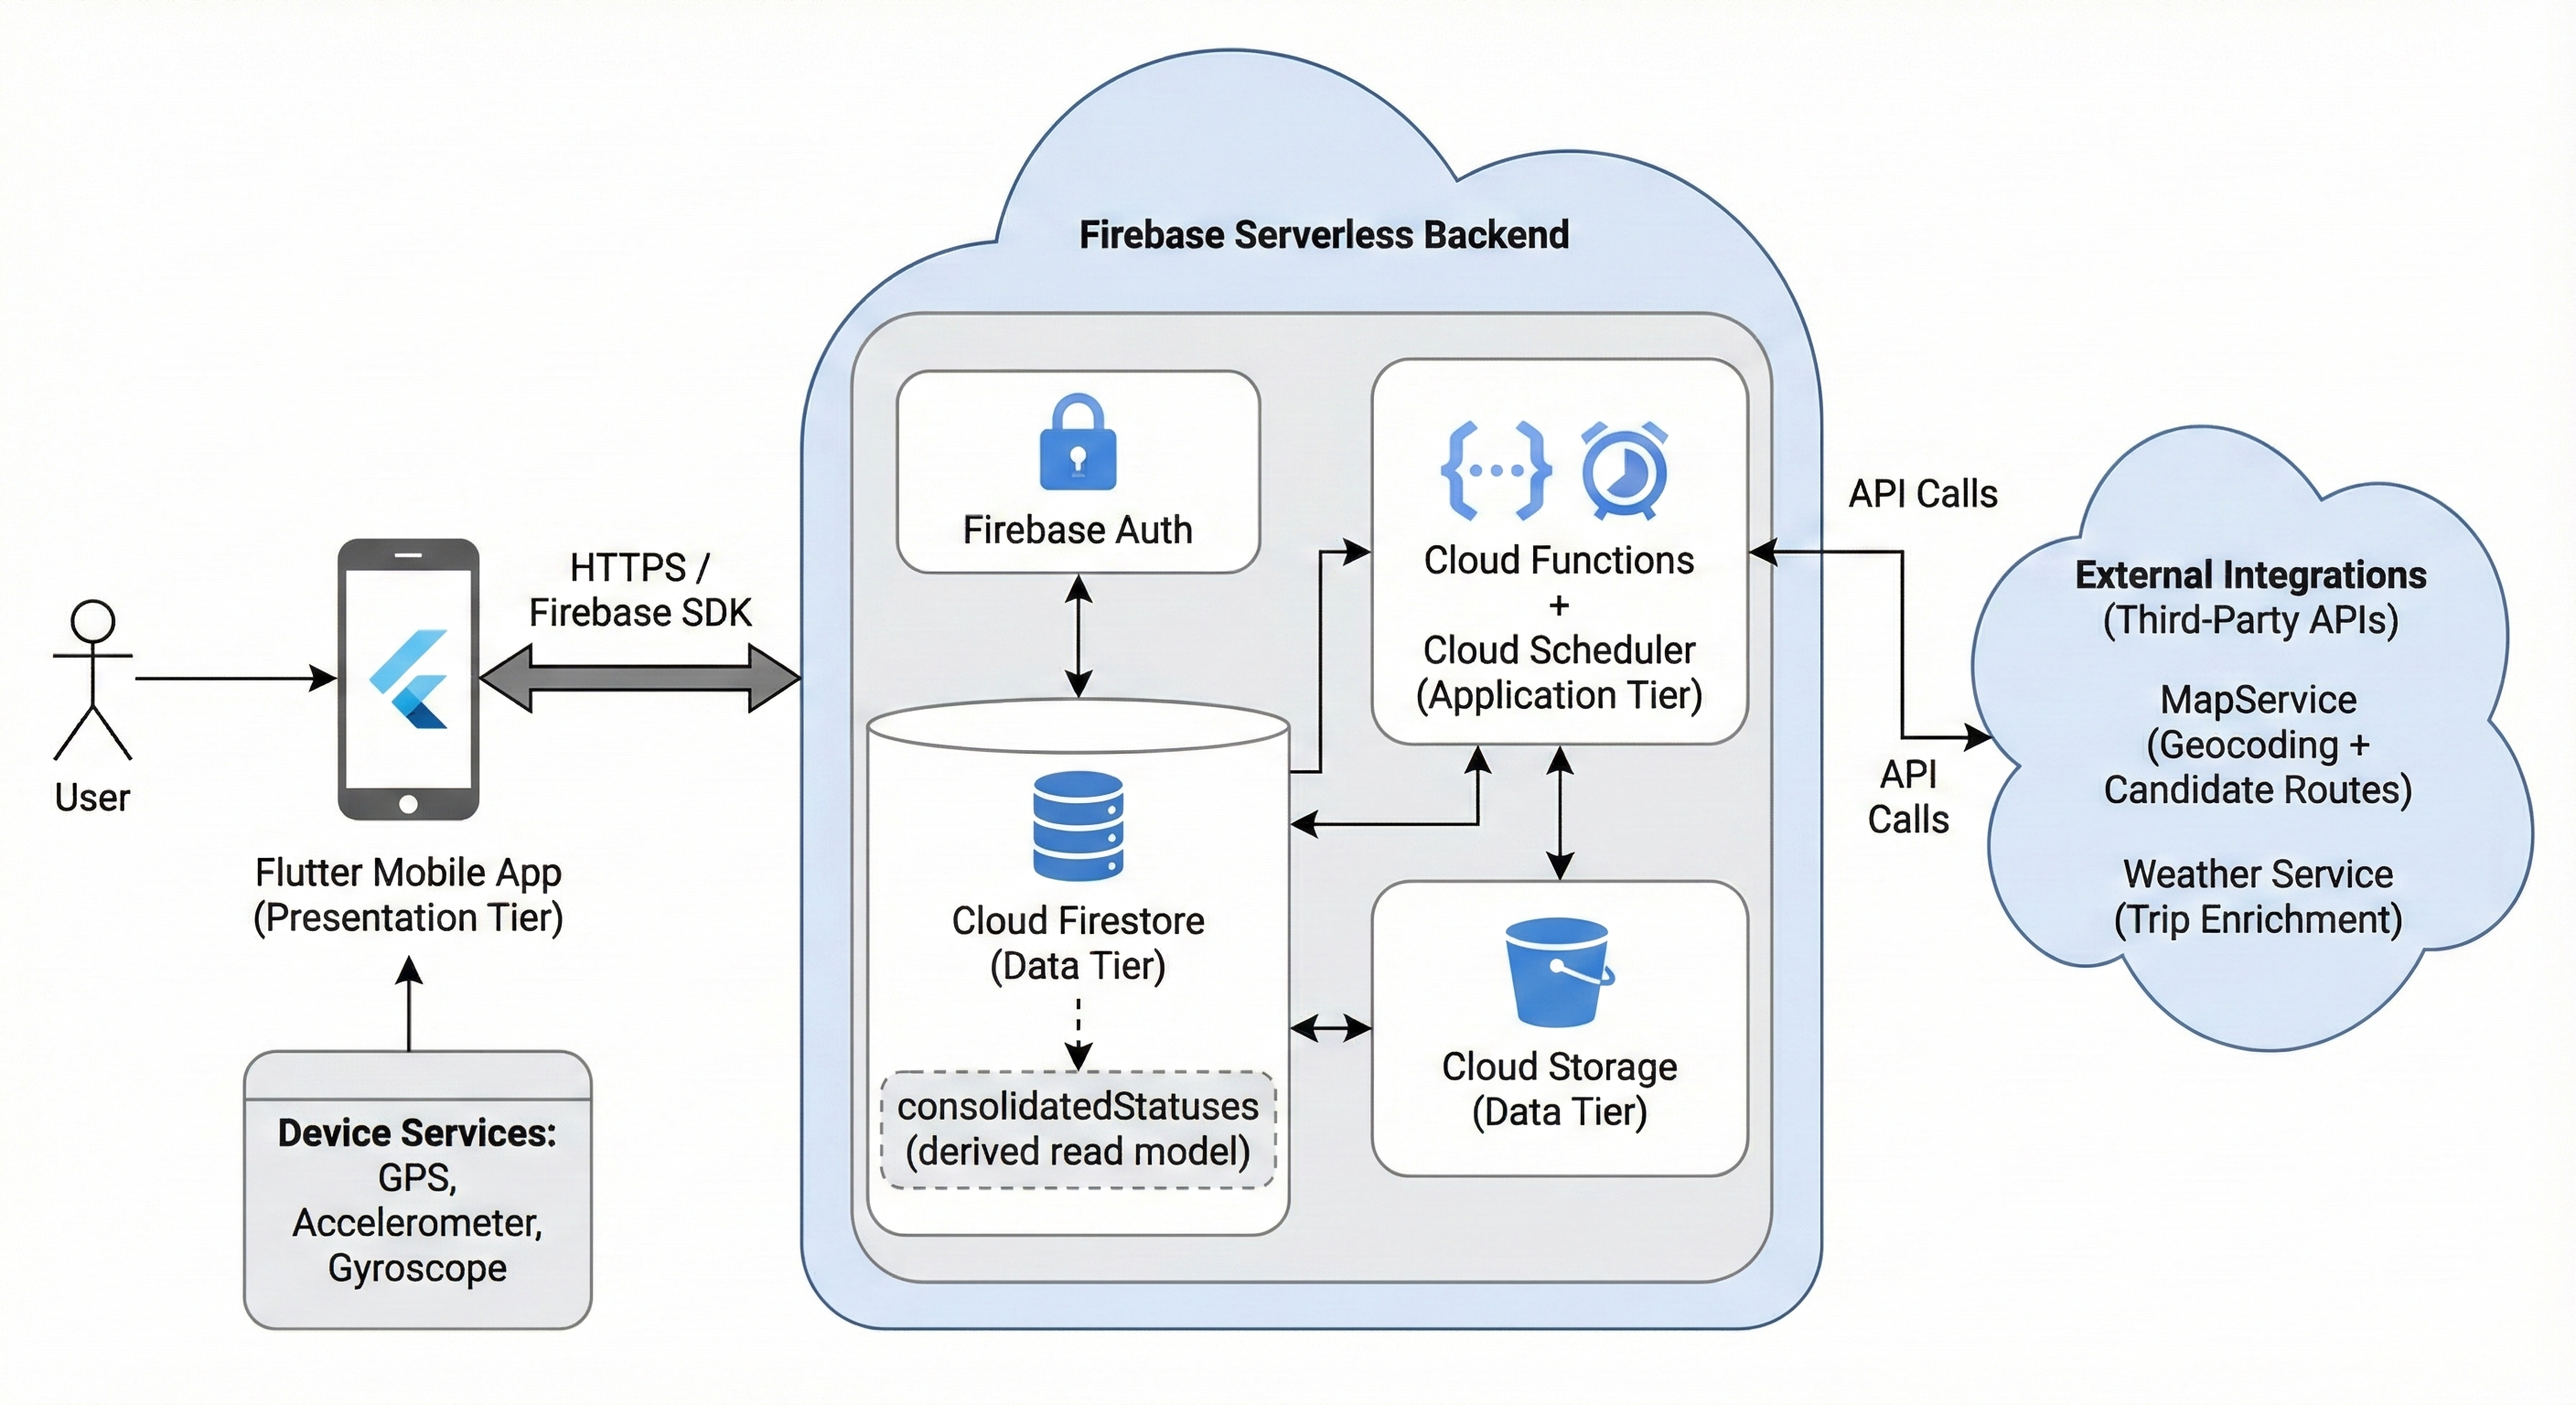
\includegraphics[width=\textwidth]{Images/Architectural overview.png}
\caption{\label{fig:architecutral_dig} Architectural Overview Diagram}
\end{figure}


\newpage

\subsection{Component View}
The system is organized into the following main components.

\begin{enumerate}
    \item \textbf{Flutter Mobile App (Presentation Tier)}: The Flutter client provides the user interface for registration and login, trip recording, contribution submission and route search. It interacts with Firebase services through the Firebase SDK over HTTPS. It also accesses device services such as GPS, accelerometer and gyroscope to collect trip traces and sensor signals that can support automatic detection workflows.

    \item \textbf{Firebase Authentication:}  Firebase Authentication manages user registration, login and session handling. It issues identity tokens that are used by clients to access protected backend resources according to Firestore Security Rules and Cloud Functions authorization checks.

        \begin{sidewaysfigure}
        \centering
        \includegraphics[width=\textwidth]{Images/component_view.jpg}
        \caption{\label{fig:domain_class_dig}Domain Class Diagram.}
        \end{sidewaysfigure}
    \item \textbf{Cloud Firestore (Data Tier):} Firestore stores the structured data required by BBP, including users, trips metadata, trip summaries, segment reports, obstacles, publishable flags and derived read models. Firestore is also used to support reactive UI updates where appropriate through real time listeners.
    \item \textbf{Cloud Storage (Data Tier):}  Cloud Storage stores larger objects, compressed location sequences and optional media attachments related to reports. Firestore stores references and metadata for these objects.
    \item \textbf{Cloud Functions and Cloud Scheduler (Application Tier):} Cloud Functions implement protected operations such as route scoring, report merging and generation of consolidated segment status. Functions also act as a controlled gateway to external services to prevent exposing API keys and to ensure consistent validation and rate limiting. Cloud Scheduler is used to trigger periodic maintenance and aggregation tasks such as recomputing consolidated statuses or cleaning up temporary records.
    \item \textbf{External Integrations (Third Party APIs):} BBP integrates with a map service for geocoding and route candidate generation between origin and destination. It also integrates with a weather service to enrich recorded trips with contextual conditions such as temperature, wind and precipitation.

\end{enumerate}


% \begin{figure}[H]
% \centering
% \includegraphics[width=\textwidth]{Images/component_view.jpg}
% \caption{\label{fig: component_dig} Component Diagram}
% \end{figure}






\newpage
\subsection{Deployment View}

BBP is deployed as a client serverless system.

\begin{enumerate}
    \item The Flutter application runs on end user mobile devices and communicates with Firebase over HTTPS using the Firebase SDK.

    \item The backend is deployed entirely on Firebase and Google Cloud managed infrastructure. Firestore and Cloud Storage store data, while Cloud Functions provide execution environments for application logic.
    \item External services are accessed by Cloud Functions, not directly by the mobile client, for operations that require secrets or controlled execution.

\end{enumerate}
This deployment minimizes backend administration, enables elastic scaling and supports a pay per use model.

\begin{figure}[H]
\centering
\includegraphics[width=0.35\textwidth]{Images/Deployment_view.png}
\caption{\label{fig:deployemnt_dig} Deployment Diagram} 
\end{figure}



\newpage
\subsection{Runtime View}
The runtime behavior of BBP can be described by considering how components collaborate to realize the core use cases.(UC1 to UC2)

\begin{enumerate}

    \item \textbf{User authentication and session establishment(UC1, UC2)}

        \begin{figure}[H]
        \centering
        \includegraphics[width=\textwidth]{Images/sequence_diagrams/UC1_page-0001.jpg}
        \caption{\label{fig:seqence_dig1} User Authentication Sequence Diagram}
        \end{figure}


        \begin{figure}[H]
        \centering
        \includegraphics[width=\textwidth]{Images/sequence_diagrams/UC2_page-0001.jpg}
        \caption{\label{fig:sequence_dig2} User Session Establishment Sequence Diagram}
        \end{figure}
    \begin{itemize}
        \item The user registers or logs in through the Flutter application.

        \item Firebase Authentication verifies credentials and returns an identity token.
        \item The client uses the token to access Firestore documents and callable or HTTPS Cloud Functions.
        

    \end{itemize}

    \item \textbf{Trip recording and storage(UC3)}
    \begin{itemize}
        \item The user starts trip recording in the Flutter application.
        \item The client reads GPS and sensor data at configured intervals.
        \item During recording, the client may compute lightweight statistics locally and stores intermediate data in memory.
        \item At the end of the trip, the client uploads trip metadata to Firestore and uploads the heavier trace payload to Cloud Storage.
        \item A Cloud Function may be triggered to compute additional derived statistics or to normalize trip structures for later visualization.
        
        \begin{figure}[H]
        \centering
        \includegraphics[width=0.65\textwidth]{Images/sequence_diagrams/UC3_page-0001.jpg}
        \caption{\label{fig:sequence_dig3} Trip Recording Sequence Diagram}
        \end{figure}


    \end{itemize}
    \item \textbf{Manual contribution workflow(UC4)}
    \begin{itemize}
        \item A registered user submits a path segment status or obstacle through the UI.
        \item The client writes the report into Firestore with a publishable flag selected by the user.
        \item A backend function validates the submission and may trigger aggregation updates for the affected segment.

        \begin{figure}[H]
        \centering
        \includegraphics[width=0.8\textwidth]{Images/sequence_diagrams/UC4_page-0001.jpg}
        \caption{\label{fig:sequence_dig4} Manual Contribution Workflow Sequence Diagram}
        \end{figure}
        
    \end{itemize}
    \item \textbf{Sensor assisted detection confirmation(UC5)}
    \begin{itemize}
        \item While recording, the client can detect candidate issues based on sensor signals and location context.
        \item Candidate issues are stored as private draft items for the user.
        \item The application prompts the user to confirm, correct or discard each candidate issue.
        \item Only confirmed and publishable items are written to the community visible collections.
        
        \begin{figure}[H]
        \centering
        \includegraphics[width=0.8\textwidth]{Images/sequence_diagrams/UC5_page-0001.jpg}
        \caption{\label{fig:sequence_dig5} Sensor Assisted Detection Confirmation Sequence Diagram}
        \end{figure}

    \end{itemize}
    \item \textbf{Route search, scoring and visualization(UC6)}
    \begin{itemize}
        \item The user specifies origin and destination in the Flutter application.
        \item The client requests candidate routes via a protected Cloud Function.
        \item The Cloud Function calls the external map service to obtain candidate routes and associated polyline or segment representations.
        \item The backend retrieves consolidated segment information from Firestore and computes a route score that combines quality and effectiveness factors.
        \item The ranked routes are returned to the client for visualization and selection.
        \item Generally, this behaviour reflects the formal cycling route research where candidate paths are ranked. Usually by a combined utility or attractiveness objective and sometimes under constraints. BBP implements a practical real time version of this idea for end users \cite{polimi_research_paper}.

        \begin{figure}[H]
        \centering
        \includegraphics[width=0.65\textwidth]{Images/sequence_diagrams/UC6_page-0001.jpg}
        \caption{\label{fig:sequence_dig6} Route Search and Scoring Sequence Diagram}
        \end{figure}

    \end{itemize}
    \item \textbf{Merging and consolidated status updates(UC7)}
    \begin{itemize}
        \item When multiple reports affect the same segment, a backend function computes a consolidated status by applying freshness and confirmation logic.
        \item The consolidated read model is stored in a dedicated collection for efficient querying during route scoring and map rendering.
        \item Periodic recomputation may be scheduled via Cloud Scheduler to ensure consistency and to incorporate aging policies.
    
        \begin{figure}[H]
        \centering
        \includegraphics[width=\textwidth]{Images/sequence_diagrams/UC7_page-0001.jpg}
        \caption{\label{fig:sequence_dig7} Merging and Consolidated Status Update Sequence Diagram}
        \end{figure}
    \end{itemize}

\end{enumerate}



\subsection{Interface View}
BBP exposes interfaces between the client and the backend through Firebase SDK operations and Cloud Functions endpoints.

\begin{enumerate}
    \item \textbf{Client to Firebase Authentication:} Registration, login, password reset and token management are handled through the Firebase SDK.
    \item \textbf{Client to Firestore:} The client reads and writes documents according to Security Rules. Typical reads include user profile, trip list, trip summaries and route results. Typical writes include trip metadata, user preferences and user owned contribution drafts.
    \item \textbf{Client to Cloud Functions:} Cloud Functions provide APIs for operations requiring server side enforcement or third party integrations such as:
        \begin{itemize}
            \item Requesting candidate routes and performing route scoring
            \item Triggering consolidation and merge processes
            \item Performing validation and normalization of submissions
            \item Retrieving weather enrichment for trips when needed
        \end{itemize}
    \item \textbf{Cloud Functions to External APIs:} Cloud Functions call map and weather services using secure stored credentials. Responses are transformed into BBP domain structures before being persisted or returned.
\end{enumerate}




\subsection{Architectural Style and Patterns}
BBP adopts the following architectural styles and patterns:
\begin{enumerate}
    \item \textbf{Serverless architecture:} The backend relies on managed services and function based computation. This supports scalability and reduces infrastructure management.
    \item \textbf{Layered architecture:} Presentation logic resides on the Flutter client, application logic resides in Cloud Functions and persistence is handled by Firestore and Cloud Storage.
    \item \textbf{Event driven and reactive data access:} Firestore enables real time updates for relevant UI elements. Backend functions may be triggered by database events to update derived models.
    \item \textbf{CQRS inspired read models:} Consolidated segment status is stored in a dedicated collection as a derived read model optimized for frequent route scoring queries. This reduces repeated computation during interactive route searches.
\end{enumerate}

\subsection{Data Management}

BBP stores and manages data in a way that supports both personal trip logs and community maintained path quality.
\begin{enumerate}
    \item \textbf{Core entities stored in Firestore}
    \begin{itemize}
        \item Users and preferences
        \item Trips metadata and summary statistics
        \item Segment reports and obstacle reports with publishable or private designation
        \item Consolidated segment statuses used for scoring and map visualization
    \end{itemize}
    \item \textbf{Large payloads stored in Cloud Storage}
    \begin{itemize}
        \item Full GPS traces and dense samples
        \item Optional attachments related to reports
    \end{itemize}
    \item \textbf{Derived read models:} Consolidated segment statuses are maintained in a separate collection to support low latency reads during route scoring. Updates occur when new publishable reports arrive and may also be recomputed periodically.
    \item \textbf{Consistency model:} Firestore provides strong consistency for document reads, while derived models may be eventually consistent depending on trigger timing. The design prioritizes user facing responsiveness, while ensuring that consolidation logic converges to stable results.
\end{enumerate}





\subsection{Security Design}

Security is enforced through a combination of authentication, authorization rules and controlled server side execution.

\begin{enumerate}
    \item \textbf{Authentication:} Users authenticate through Firebase Authentication. Identity tokens are required for operations tied to personal data or contributions.
    \item \textbf{Authorization:} Firestore Security Rules restrict reads and writes based on user identity and ownership. Private trip data and private candidate issues are accessible only to their owners. Community visible publishable data is readable according to the intended visibility rules.
    \item \textbf{Protected operations:} Cloud Functions encapsulate operations that require secrecy, controlled validations or merging logic. External API keys are not embedded in the client.
    \item \textbf{Privacy by design:} The system maintains a strict separation between private user data and publishable community data. Publication is always an explicit user choice.
\end{enumerate}



\subsection{Design Decisions and Rationale}
The chosen architecture reflects the project constraints and the expected usage patterns.


\begin{enumerate}
    \item Firebase services provide a consistent ecosystem for authentication, real time data access and secure server side logic, reducing integration complexity.
    \item Cloud Functions centralize business rules such as merging and scoring, which improves integrity and prevents client side manipulation.
    \item The use of a consolidated status read model improves performance during route searches by avoiding expensive aggregation at query time.
    \item Cloud Storage is used for large traces to keep Firestore efficient and to reduce document size constraints.
    \item External API calls are handled server side to protect secrets, manage quotas and provide a stable contract to the client.
\end{enumerate}
